\chapter{Modelling} \label{cha:chapter-3}

\section{Results}

For the modelling, the data was split into train and test sets with proportions 0.7 and 0.3 respectively. The bad rate was maintained in each data at 17\% to ensure fairness and the variables were converted to their woe values for their respective bin from tables  (\ref{woe_1}) \& (\ref{woe_2}). Once split the train data was passed through a glm model with logit link, for this the python package statsmodels was used \cite{statsmodels}. Three models were created, first was the base model with every variable included with no changes. For the second model I looked at applying log transformations to the variables which had a heavy right skew, LOAN, MORTDUE, VALUE and YOJ. These values were then passed through the woe binning and the values converted. The IV of LOAN and YOJ improved by 0.01 and 0.03 respectively whilst MORTDUE and VALUE's IV decreased, based on this only the log transformations of LOAN and YOJ were kept and used for the second model. Finally, a third model was made from dropping variables with high p-values, these were MORTDUE and REASON. \\

The results for each of these models can be found in the appendix (), () and (). The performance of each model is shown and compared in Table (\ref{perf_eval}). It can be seen from this table that based on the performance evaulation mentioned in Section \ref{sec:perf_eval}. Model 2 and 3 appear to out perform Model 1 but when comparing the two the difference between performance indicators becomes smaller. In the case of Model 3 the AIC is lower but the GINI coefficient is also lower than Model 2. Based on Table (\ref{perf_eval}) either Model 2 or 3 would be an appropriate choice but I decided to go with Model 2. This is because the difference in AIC is only 3.26 and when looking at the Log-Likelihood for each model the difference is 0.4. This is implying that the performance based on AIC is only better because of the removal of two variables making it a smaller and less complicated model. Where as the GINI coefficient doesn't consider the complication of the model. \\

In figure (\ref{scorecard_plot}) the results from the logisitc regression have been used and converted into a scorecard. The figure displays the distribution and bad probability for the test and train data sets. You can see the distributions follow each other nicely but when looking at the bad probability, the probability of each bin follows the same trend excluding the bin [350, 400). Looking further into this it appears.

\begin{figure}
\begin{center}
\renewcommand{\arraystretch}{1.25}
\begin{tabular}{lcccc}
\toprule
Model & AIC & KS & GINI & Potential Loss \\
Model 1 (Default) & 2491.73 & 0.4892 & 0.6156 & \$0 \\
Model 2 (Log transformations) & 2460.77 & 0.4890 & 0.6186 & \$0 \\
Model 3 (REASON and MORTDUE dropped) & 2457.51 & 0.4858 & 0.6180 & \$0 \\
\bottomrule
\end{tabular}
\caption{Performance Evaluation Results On Test \label{perf_eval}}
\end{center}
\end{figure}

\begin{figure}[!ht]
	\centering
	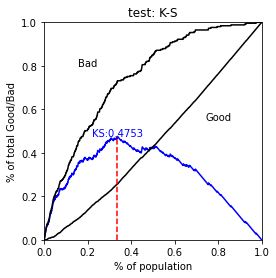
\includegraphics[scale=0.90]{figs/ks_plot.png}
	\caption{KS Plot \label{ks_plot}}
\end{figure}

\begin{figure}[!ht]
	\centering
	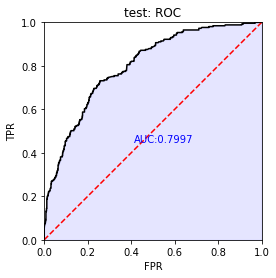
\includegraphics[scale=0.90]{figs/roc_plot.png}
	\caption{ROC Plot \label{roc_plot}}
\end{figure}

\begin{landscape}
\begin{figure}[!ht]
\begin{center}
	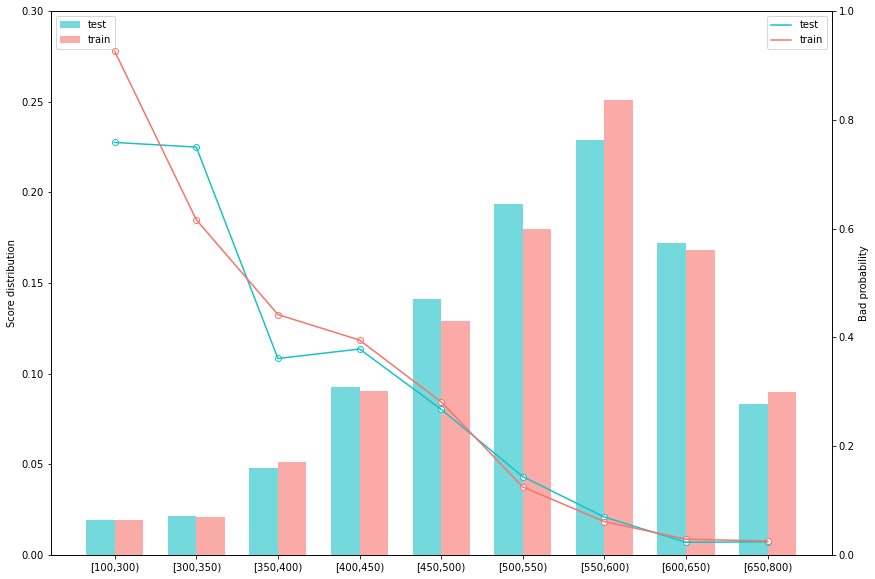
\includegraphics[scale=0.70]{figs/scorecard_plot.png}
	\caption{Scorecard Plot \label{scorecard_plot}}
\end{center}
\end{figure}
\end{landscape} 
